\documentclass[12pt]{article}
\usepackage{../../template}
\title{Lecture 8}
\author{niceguy}
\begin{document}
\maketitle

\section{Twitch vs Mixer}
Let $x(t)$ and $y(t)$ be the users on Twitch and Mixer respectively. We assume
\begin{itemize}
	\item For every existing user on Twitch, Twitch gains 2 more users
	\item For every existing user on Mixer, Mixer gains 4 more users
	\item Twitch loses 1 viewer for every viewer on Mixer
	\item Mixer loses 3 viewers for every viewer on Twitch
	\item Twitch naturally gains 200 new viewers
	\item Mixer naturally gains 50 new viewers
\end{itemize}

What will happen to both platforms?
$$\frac{dx}{dt} = 2x-y+200$$
$$\frac{dy}{dt} = 4y-3x+50$$
This can be rewritten as
$$\begin{pmatrix} x' \\ y' \end{pmatrix} = \begin{pmatrix} 2 & -1 \\ -3 & 4 \end{pmatrix} \begin{pmatrix} x \\ y \end{pmatrix} + \begin{pmatrix} 200 \\ 50 \end{pmatrix}$$

\begin{figure}
	\centering
	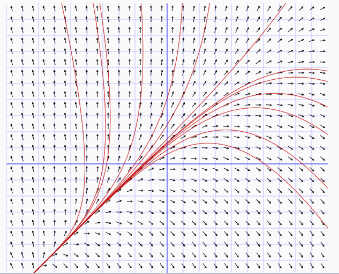
\includegraphics[width=\textwidth]{phasepotraita.png}
	\caption{Phase Potrait (stolen from Beamer Slides)}
	\label{pota}
\end{figure}

Based on the phase potrait (Fig \ref{pota}), it is possible for both Twitch and Mixer to succeed. However, in reality, Mixer failed.

\begin{defn}
	A first order linear system of ODEs of dimension two is given by
	$$\begin{pmatrix} x' \\ y' \end{pmatrix} = \begin{pmatrix} p_{11}(t) & p_{12}(t) \\ p_{21}(t) & p_{22}(t) \end{pmatrix} \begin{pmatrix} x \\ y \end{pmatrix} + \begin{pmatrix} g_1(t) \\ g_2(t) \end{pmatrix}$$
	If $g_1(t) = g_2(t) = 0$, this system is called homogeneous.
\end{defn}

\begin{thm}
	Suppose we have a first order linear system of ODEs as defined above with the initial conditions
	$$\begin{pmatrix} x(t_0) \\ y(t_0) \end{pmatrix} = \begin{pmatrix} x_0 \\ y_0 \end{pmatrix}$$
	Let $I = (\alpha, \beta)$ be the largest interval satisfying
	\begin{itemize}
		\item $t_0 \in I$
		\item $p_{11}(t), p_{12}(t), p_{21}(t), p_{22}(t)$ are all continuous on $I$
		\item $g_1(t)$ and $g_2(t)$ are continuous on $I$
	\end{itemize}
	Then the initial value problem has a unique solution defined on all of $I$.
\end{thm}

Therefore, for autonomous systems, where all $p$ and $g$ are independent of $t$ (i.e. constants), we are guaranteed a unique solution for $t \in \R$. (The proof is trivial and is left to the reader as an exercise)

\section{Twitch Partnerships}

Twitch also forms partnerships. Say Twitch partners with Apex Legends. We assume
\begin{itemize}
	\item For every Apex player, Twitch gains one new subscriber
	\item For every two Twitch users, Apex gains one player
\end{itemize}

Let's consider a setting where both are losing consumers due to school
\begin{itemize}
	\item For every user on Twitch, Twitch loses 2 more users
	\item For every player on Apex, Apex loses 2 more players
\end{itemize}

Despite the losses, they still gain a fixed number of users/players
\begin{itemize}
	\item Twitch still gains a consistent 200 viewers
	\item Apex still gains a consistent 20 players
\end{itemize}
Then the system becomes
$$\begin{pmatrix} x' \\ y' \end{pmatrix} = \begin{pmatrix} -2 & 1 \\ 0.5 & -2 \end{pmatrix} \begin{pmatrix} x \\ y \end{pmatrix} + \begin{pmatrix} 200 \\ 20 \end{pmatrix}$$

\begin{figure}
	\centering
	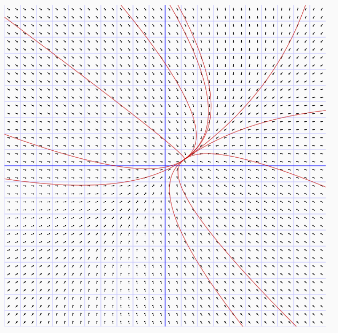
\includegraphics[width=\textwidth]{phasepotraitb.png}
	\caption{Phase Potrait (also stolen from Beamer)}
	\label{potb}
\end{figure}

By observation (Fig \ref{potb}), the solutions converge to a point. This gives us
$$\begin{pmatrix} 0 \\ 0 \end{pmatrix} = \begin{pmatrix} -2 & 1 \\ 0.5 & -2 \end{pmatrix} \begin{pmatrix} x \\ y \end{pmatrix} + \begin{pmatrix} 200 \\ 20 \end{pmatrix}$$
Solving this, we have
$$\begin{pmatrix} x \\ y \end{pmatrix} = \begin{pmatrix} 120 \\ 40 \end{pmatrix}$$
\end{document}
